\documentclass[resume]{subfiles}

\begin{document}
\section{Bootloader}

\begin{itemize}
\item C'est une application (logiciel)
\item Permettre à un software/firmware d'être mis à jour
\item Sans l'utilisation d'un hardware spécialisé(No Jtag prog)
\item Différents protocoles pour recevoir le software update
\end{itemize}

\begin{figure}[H]
    \centering
    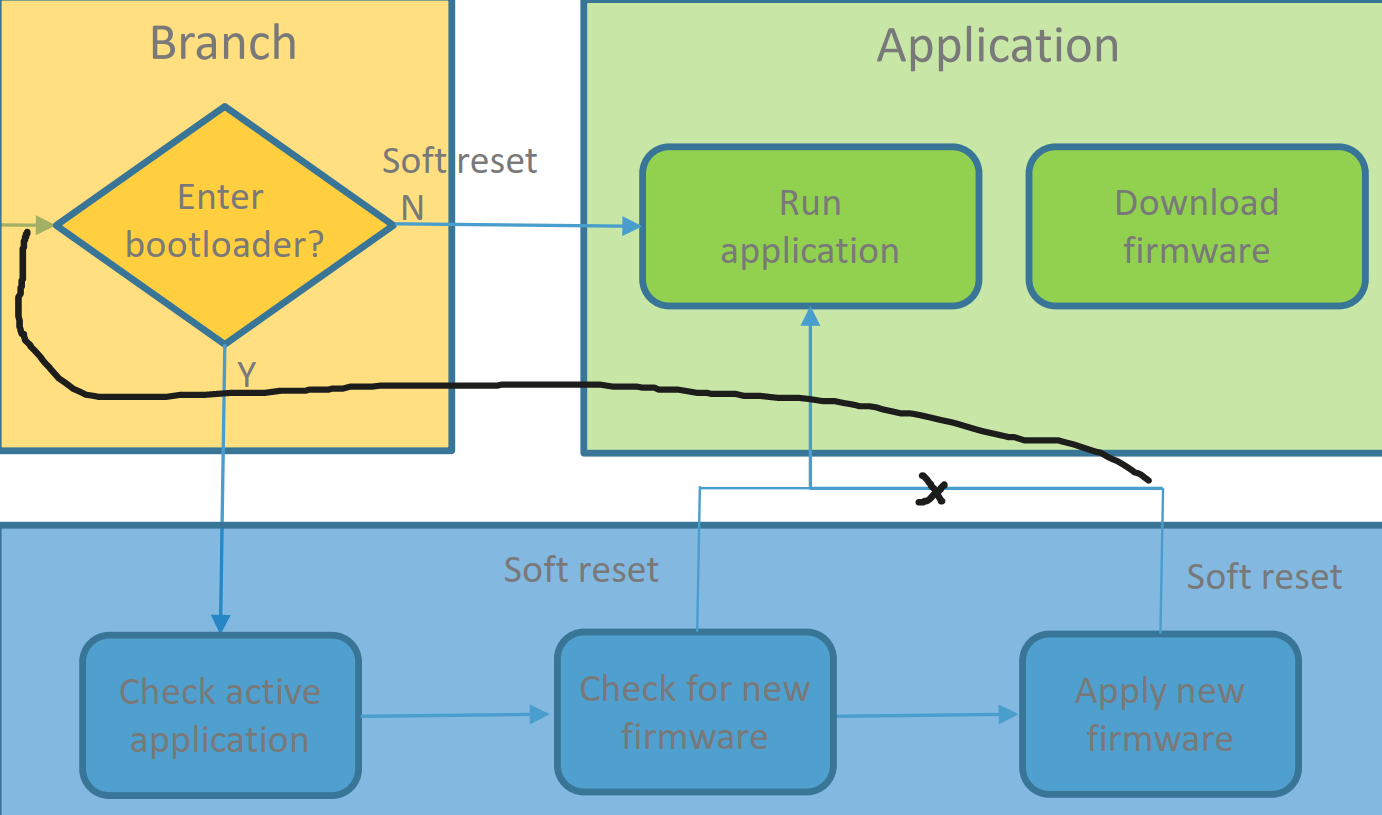
\includegraphics[width=0.6\columnwidth]{Figures/bootloader/schemaBloc.png}
\end{figure}
Vector table, bootloader, application, candidat(nouvelle application)
\end{document}